%
\begin{table}[h]
	\resizebox{1.01\columnwidth}{!}{%
		\centering\begin{tabular}{clcclllc}\toprule
			&        &                         &                         & Quality   & Protected & Protected \\
			& Dataset & \multicolumn{1}{c}{$n$} & \multicolumn{1}{c}{$k$} & criterion & groups     & \% \\ 
			\midrule
			D1 & COMPAS \cite{angwin_2016_machine}& 6173 & 1500 & ad-hoc score & PoC & 65.9\% \\
			\midrule
			D2 & COMPAS \cite{angwin_2016_machine}& 6173 & 500 & ad-hoc score & < 25yr. & 21.8\% \\
			& & & & & 25yr. < x < 45yr. & 57.2\% \\
			\midrule
			D3 & COMPAS \cite{angwin_2016_machine}& 6173 & 500 & recidivism + & PoC female, < 25yr. & 2.8\%\\ 
			& & & & prior arrests + & white female, < 25yr. & 1.2\% \\
			& & & & violent recidivism & PoC male, < 25yr. & 13.4\% \\
			\midrule
			D4 & German credit \cite{lichman_2013_uci} & 1000 & 100 & credit rating & female, non-prot. age & 21.7\% \\
			& & & & & male, oldest 10\% & 6.3\% \\
			& & & & & female, youngest 10\% & 6.1\% \\
			& & & & & male, youngest 10\% & 4.4\% \\
			& & & & & female, oldest 10\% & 3.2\% \\
			\midrule
			D5 & LSAT \cite{wightman1998lsac}  & 21K & 500  & LSAT score  & White, female & 35.3\%  \\ 
			& & & & & PoC, female & 8.4\% \\
			& & & & & PoC, male & 7.6\% \\
			\bottomrule
		\end{tabular}
	}
	\caption{Datasets and experimental settings.	\label{tbl:datasets}}
	\vspace{-3mm}
\end{table}
%
\section{Experiments}\label{sec:experiments}
%\todo{Are we still doing this experiment to verify algorithm correctness?}
%In the first part of our experiments we create synthetic datasets to demonstrate the correctness of the adjustment done by Algorithm \algoCorrect (\S\ref{subsubsec:JuliaExperimentalVerification}).
%
In this section, we consider several public datasets for evaluating the multinomial \algoFAIR algorithm (datasets in \S\ref{sec:experiments-datasets}, metrics and comparison with baselines in \S\ref{sec:experiments-baselines}, and results in \S\ref{sec:experiments-results}).

\begin{figure}[t]
	\vspace{-8mm}
	\centering
	\subfloat%
	[Score distribution of male and female candidates in the COMPAS dataset.
	\label{fig:dataset:compas:sex}]
	{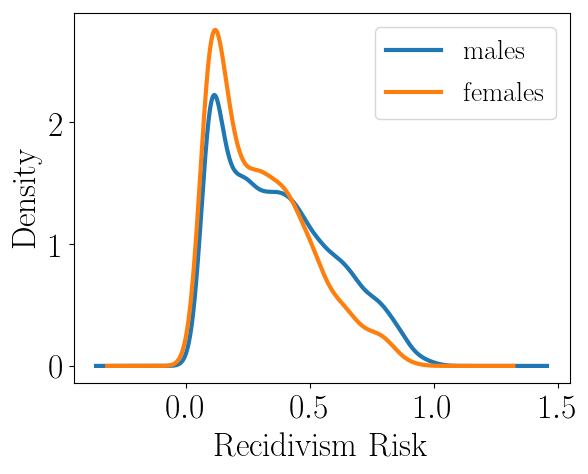
\includegraphics[width=.48\textwidth]{pics/compas_sex_kde.png}}\hfill
	\subfloat
	[Score distribution of white and non-white candidates in the COMPAS dataset. Experiment D1.
	\label{fig:dataset:compas:race}]
	{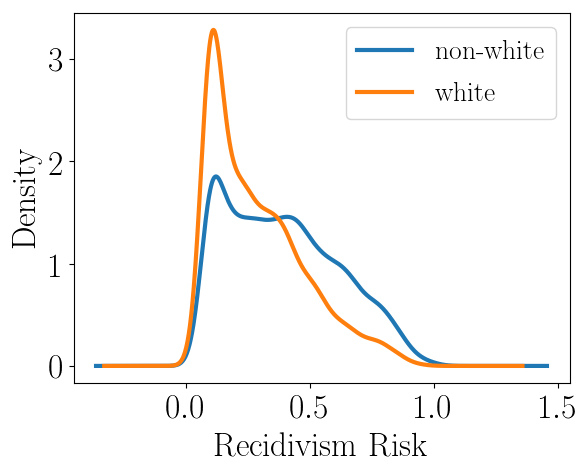
\includegraphics[width=.48\textwidth]{pics/compas_race_kde.png}}\hfill
	\subfloat
	[Score distribution by age in the COMPAS dataset. We see that age is a strong predictor of recidivism risk which suggests that the COMPAS questionnaire injects a bias against younger people into the data. Experiment D2.
	\label{fig:dataset:compas:age}]
	{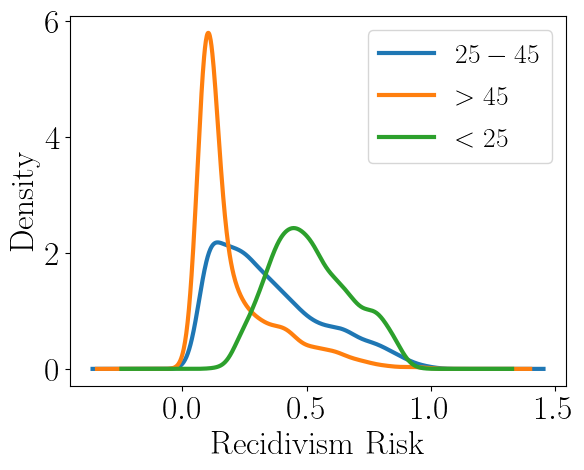
\includegraphics[width=.48\textwidth]{pics/compas_age_kde.png}}\hfill
	\subfloat
	[Score distribution protected and non-protected candidates in the COMPAS dataset. Protected groups are young non-white males, young non-white females and young white females, which are the three groups with lowest average exposure in the colorblind ranking. Experiment D3.
	\label{fig:dataset:compas:worstThree}]
	{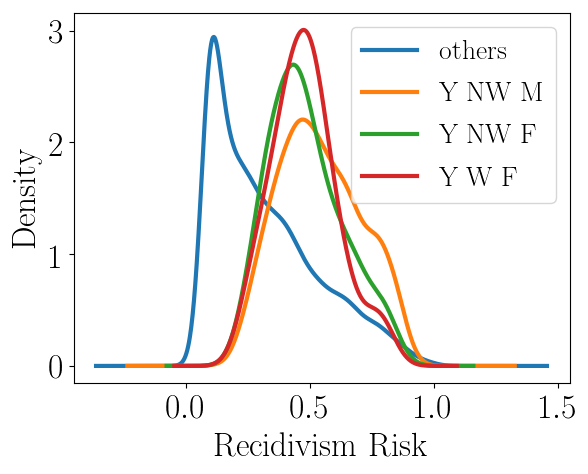
\includegraphics[width=.48\textwidth]{pics/compas_worstThreeGroups_kde.png}}\hfill
	\vspace{-3mm}
	\caption{Distribution of COMPAS scores in different experimental settings. The first three figures show distributions separately by each of the three protected categories. The fourth figure shows the distribution for dataset D3}
	\label{fig:dataset:compas}
	\vspace{-3mm}
\end{figure}

\subsection{Datasets}\label{sec:experiments-datasets}

Table~\ref{tbl:datasets} summarizes the datasets used in our experiments.
%
Each dataset contains a set of people with demographic attributes, plus a quality attribute.
%
Note that dataset D1 is the same experimental setup as in our previous paper~\cite{zehlike2017fair}, but instead of using the original algorithm \algoFAIR, we run the binomial experiment with the multinomial extension proposed in Section~\ref{sec:problem}.
%
For each dataset, we consider a value of $k$ that is a round number ({\em e.g.}, 100, or 500) with $k<n$.
%
For the purposes of these experiments, we considered several scenarios of protected groups.
%
We remark that the choice of protected group is not arbitrary: it is determined completely by law or voluntary commitments; for the purpose of experimentation we test different scenarios, but in a real application there is no ambiguity about which is the protected group and what is the minimum proportion.
%
An experiment consists of generating a ranking using multinomial \algoFAIR and then comparing it with baseline rankings according to the metrics introduced in the next section.
%
We use the three publicly-available datasets: COMPAS~\cite{angwin_2016_machine}, German Credit~\cite{lichman_2013_uci}) and LSAC~\cite{wightman1998lsac}.

\spara{COMPAS} (Correctional Offender Management Profiling for Alternative Sanctions) is an assessment tool for predicting recidivism based on a questionnaire of 137 questions. It is used in several jurisdictions in the US, and has been accused of racial discrimination by producing a higher likelihood to recidivate for African Americans~\cite{angwin_2016_machine}.
%
In our experiment, we test a scenario in which we want to create a fair ranking of the top-$k$ people who are least likely to recidivate, who could be, for instance, considered for a pardon or reduced sentence.
%
We calculated a candidate's overall score as a weighted summation of the columns ``recidivism, violent recidivism'' and ``prior arrests'' from the original dataset.
%
Our protected groups are formed by different combination of the attributes ``race, age'' and ``sex'', where race is either ``white'' or ``non-white'', age is either ``younger than 25'', ``between 25 and 45'' or ``older than 45'', and sex is either ``male'' or ``female''.
%
We observe in Figure~\ref{fig:dataset:compas} that non-white people (\ref{fig:dataset:compas:race}), as well as males (\ref{fig:dataset:compas:sex}) are given a larger recidivism score than other groups.
%
However we see in Figure~\ref{fig:dataset:compas:age} that the protected attribute ``age'' has the strongest impact on recidivism risk. 
%
Apparently the questionnaire imposes a strong bias against younger people.
%
We therefore consider white, female and older than 45 as the \emph{non-protected} categories for our experiments.
%
In dataset D3 we divided the candidates into 12 different groups that we constructed from the Cartesian product of all three protected categories ``age, race'' and ``sex''. 
%
Then we calculated the average group exposure for each group and declared those three groups as protected that were placed lowest in the colorblind ranking.
%
These are young non-white females, young white females and young non-white males.
%
Interestingly, despite the fact that females have higher scores on average, two of the three groups with lowest exposure values are female (Figure~\ref{fig:dataset:compas:worstThree}).

\spara{German Credit} is the Statlog German Credit Data collected by Hans Hofmann~\cite{lichman_2013_uci}.
%
It is based on credit ratings generated by Schufa, a German private credit agency based on a set of variables for each applicant, including age, gender, marital status, among others. The Schufa score is an essential determinant for every resident in Germany when it comes to evaluating credit rating before getting a phone contract, a long-term apartment rental or almost any loan.
%
We use the credit-worthiness as qualification, calculated as a weighted summation of the features account status, credit duration, credit amount and employment length. 
As protected attributes we use the sex and age of a candidate: females and whether or not they belong to the group of the 100 youngest or oldest persons respectively form the protected groups, because these tend to be given lower scores.

\spara{LSAT} is a dataset collected by~\citet{wightman1998lsac} to study whether the admission metrics to law schools in the US disadvantage students of color. 
%
The qualification attribute consists of scores in the US Law School Admission Test.
%
The protected features are a person's sex and whether or not they belong to the group of people of color (PoC).
%
Women and PoC score on average lower than men and Whites in this dataset, which is why we regard white men as non-protected and the other groups as protected.

\subsection{Baselines and Metrics}\label{sec:experiments-baselines}

For each dataset, we generate various top-$k$ rankings with varying targets of minimum proportion of protected candidates $p$ using \algoFAIR, plus two baseline rankings:

\spara{Baseline 1: Color-blind ranking.} The ranking $c|_k$ that only considers the qualifications of the candidates, without considering group fairness, as described in Section~\ref{concept:color-blind-ranking}.

\spara{Baseline 2: \citet{zehlike2020matching}.} The Continuous Fairness Algorithm (CFA$\theta$) is a post-processing ranking method that aligns the score distributions of the protected candidates with the Wasserstein-barycenter of all group distributions.
%
To achieve this the algorithm finds a new distribution of scoresfor each group, the "fair representation", by interpolating between the barycenter and the group distribution, subject to a given fairness parameter $\theta$.
%
This fair representation corresponds to the idea to rank groups separately and then subsequently pick the best candidates from each group to create the result ranking. 

\spara{Utility (Performance Measure). } We report the loss in ranked utility after score normalization, in which all $q_i$ are normalized to be within $[0, 1]$.
%
We also report the maximum rank drop, {\em i.e.}, the number of positions lost by the candidate that realizes the maximum ordering utility loss.

\spara{NDCG (Performance Measure). }
%
We report a normalized weighted summation of the quality of the elements in the ranking, $\sum_{i=1}^{k} w_i q_{(\tau_i)}$, in which the weights are chosen to have a logarithmic discount in the position:  $w_i = \frac{1}{\log_2 (i+1)}$. This is a standard measure to evaluate search rankings~\cite{jarvelin2002cumulated}.
%
This is normalized so that the maximum value is $1.0$.

\spara{Exposure (Fairness Measure). } We use a measure of average group exposure, which we define as the average position bias that a group is exposed to. 
%
In rankings their exposure to the user is critical for ranked candidates to benefit from the system and if a group of candidates is systematically ranked low, it can be considered as biased~\cite{friedman1996bias}. 
%
We model position bias $v$ by means of a geometric progression of the form $v(k) = \frac{1}{\log_2(i+1)}$. 
%
Thus the first position has a bias $v(1)=1$, which then decreases logarithmically.
%
Higher position bias translates into more exposure and hence more visibility.
%
We show that large increases in average group exposure can be achieved with relatively small losses in ordering utility and NDCG.

\subsection{Results}\label{sec:experiments-results}
%
\begin{table}[t]
	\caption{Experimental results, highlighting in boldface the best non-color-blind result. 
		%
		All measures are present per group except for the loss of NDCG which is calculated for the entire ranking. 
		%
		With $p_{\text{stat}}$ we denote a vector $p_G$ that contains the share of a group as its $p$-value, hence the produced ranking should obtain statistical parity.
		%
		With $p_{\text{equal}}$ we denote a vector $p_G$ that contains the same value for all $p$.
		\meike{Both FA*IR and the baseline from \citeauthor{zehlike2020matching} achieve the same target proportion of protected elements in the output and the same selection unfairness, but in general FA*IR achieves it with less ordering unfairness, and with less maximum rank drop (the number of positions that the most unfairly ordered element drops).}}
	\vspace{-3mm}
	\label{tbl:results}
	\resizebox{1.02\columnwidth}{!}{%
		\centering\begin{tabular}{llcccccc}\toprule
			&        & Exposure &   total    & Ordering     & Rank & Selection \\
			& Method & gain  & NDCG loss  & utility loss & drop & utility loss \\ \midrule
			D1, k=1500 & Colorblind & 0.0 & 1.0000 & 0.0000 & 0 & 0.0000 \\
			COMPAS, & \algoFAIR $p_{\text{stat}}$ &  & \textbf{} & \textbf{} & \textbf{} & \textbf{} \\
			race (1 prot.) & \citeauthor{zehlike2020matching} &  &  &  &  &  \\ \midrule
			D1, k=1500 & Colorblind & 0.0 & 1.0000 & 0.0000 & 0 & 0.0000 \\
			COMPAS, & \algoFAIR $p_{\text{equal}}$ &  & \textbf{} & \textbf{} & \textbf{} & \textbf{} \\
			race (1 prot.) & \citeauthor{zehlike2020matching} &  &  &  &  &  \\ \midrule
			\midrule
			
			D2, k=500 & Colorblind & 0.0 & 1.0000 & 0.0000 & 0 & 0.0000 \\
			COMPAS, & \algoFAIR $p_{\text{stat}}$ &  & \textbf{} & \textbf{} & \textbf{} & \textbf{} \\
			age (2 prot.) & \citeauthor{zehlike2020matching} &  &  &  &  &  \\ \midrule
			
			D2, k=500 & Colorblind & 0.0 & 1.0000 & 0.0000 & 0 & 0.0000 \\
			COMPAS, & \algoFAIR $p_{\text{equal}}$ &  & \textbf{} & \textbf{} & \textbf{} & \textbf{} \\
			age (2 prot.) & \citeauthor{zehlike2020matching} &  &  &  &  &  \\ \midrule
			\midrule
			
			D3, k=500 & Colorblind & 0.0 & 1.0000 & 0.0000 & 0 & 0.0000 \\
			COMPAS, & \algoFAIR  $p_{\text{stat}}$ &  & \textbf{} & \textbf{} & \textbf{} & \textbf{} \\
			age, sex, race & \citeauthor{zehlike2020matching} &  &  &  &  &  \\ \midrule
			
			D3, k=500 & Colorblind & 0.0 & 1.0000 & 0.0000 & 0 & 0.0000 \\
			COMPAS, & \algoFAIR  $p_{\text{equal}}$ &  & \textbf{} & \textbf{} & \textbf{} & \textbf{} \\
			age, sex, race & \citeauthor{zehlike2020matching} &  &  &  &  &  \\ \midrule
			\midrule
			
			D4, k=100  & Colorblind & 0.0 & 1.0000 & 0.0000 & 0 & 0.0000 \\
			German credit, & \algoFAIR $p_{\text{stat}}$ &  & \textbf{} & \textbf{} & \textbf{} & \textbf{} \\
			sex, age (5 prot.) & \citeauthor{zehlike2020matching} &  &  &  &  &  \\ \midrule
			
			D4, k=100  & Colorblind & 0.0 & 1.0000 & 0.0000 & 0 & 0.0000 \\
			German credit, & \algoFAIR $p_{\text{equal}}$ &  & \textbf{} & \textbf{} & \textbf{} & \textbf{} \\
			sex, age (5 prot.) & \citeauthor{zehlike2020matching} &  &  &  &  &  \\ \midrule
			\midrule
			
			D5, k=500  & Colorblind & 0.0 & 1.0000 & 0.0000 & 0 & 0.0000 \\
			LSAT,& \algoFAIR $p_{\text{stat}}$ &  & \textbf{} & \textbf{} & \textbf{} & \textbf{} \\
			sex, race (3 prot.) & \citeauthor{zehlike2020matching} &  &  &  &  & \textbf{} \\ \midrule
			
			D5, k=500  & Colorblind & 0.0 & 1.0000 & 0.0000 & 0 & 0.0000 \\
			LSAT,& \algoFAIR $p_{\text{equal}}$ &  & \textbf{} & \textbf{} & \textbf{} & \textbf{} \\
			sex, race (3 prot.) & \citeauthor{zehlike2020matching} &  &  &  &  & \textbf{} \\			
			\bottomrule
		\end{tabular}
	}
	\vspace{-3mm}
\end{table}
%
Table~\ref{tbl:results} summarizes the results. We report on the result using $p_G$ in two different settings, namely as a statistical parity vector i.e. the $p$-values for each group correspond to their respective proportions in the dataset and as a vector with all $p$-values being equal. 
%
First, we observe that in general changes in utility with respect to the color-blind ranking are minor, as the utility is dominated by the top positions, which do not change dramatically.
%
\meike{Revise this: Second, \algoFAIR achieves higher or equal selection utility than the baseline~\cite{zehlike2020matching} in all but one of the experimental conditions (D7).
%
Third, \algoFAIR achieves higher or equal ordering utility in all conditions. This is also reflected in the rank loss of the most unfairly
treated candidate included in the ranking ({\em i.e.}, the candidate that achieves the maximum ordering utility loss).} %, which is always equal or less for \algoFAIR.

Importantly, \algoFAIR allows to create rankings for user-defined values of $p$ and in particular for values beyond statistical parity, something that cannot be done directly with the baseline (\citet{zehlike2020matching} allows at maximum statistical parity in the result ranking when setting $\theta=1$, i.e. to the maximum value).
%
\meike{see how to plot a figure from the results: Figure~\ref{fig:results-moving-p} shows results when varying $p$ in dataset D4 (German credit, the protected group is people under 25 years old).
%
This means that \algoFAIR allows a wide range of positive actions, for instance, offering favorable credit conditions to people with good credit rating, with a preference towards younger customers.
%
In this case, the figure shows that we can double the proportion of young people in the top-$k$ ranking (from the original 15\% up to 30\%) without introducing a large ordering utility loss and maintaining NDCG almost unchanged.}

\begin{figure}[t!]
	\centering
	\subfloat[Ordering utility]{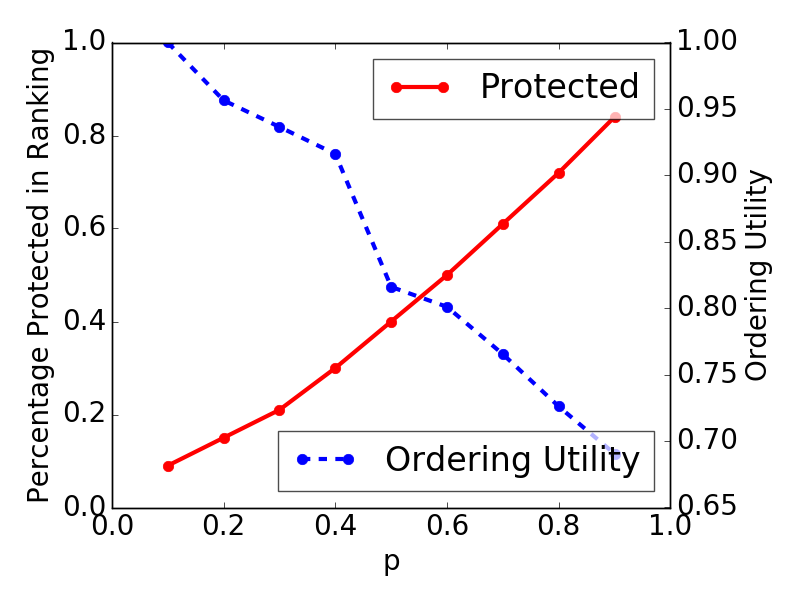
\includegraphics[width=.49\columnwidth]{pics/d4-protected-vs-ordering.png}}
	\subfloat[NDCG]{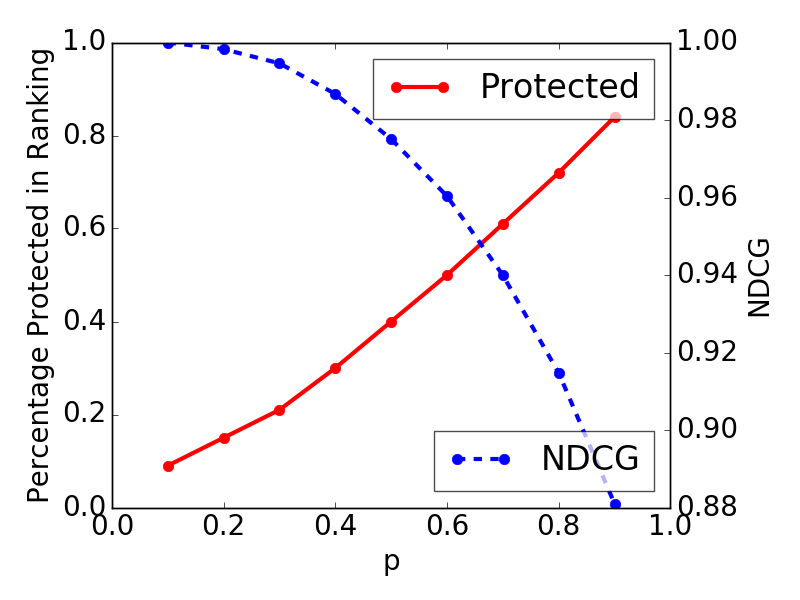
\includegraphics[width=.49\columnwidth]{pics/d4-protected-vs-ndcg.png}}
	\vspace{-2mm}
	\caption{\meike{replace figure} Depiction of possible trade-offs using \algoFAIR. Increase in the percentage of protected candidates in D5 (German credit, protected group age $<$ 25) for increasing values of $p$, compared to %decrease in ordering utility (left) and decrease in NDCG (right).}
		ordering utility and NDCG.}
	\vspace{-\baselineskip}
	\label{fig:results-moving-p}
\end{figure}
